\newpage
\section{Karty katalogowe}
\subsection{Przełącznik warstwy 3}
\textbf{Cisco Catalyst WS-C3550-12T Managed Switch 12 Ports} 
\begin{itemize}
	\item \textbf{Cisco Part Number:} WS-C3550-12T
	\item \textbf{Speed:} 10/100/1000Mbps
	\item \textbf{Flash Memory:} 8MB Memory
	\item \textbf{RAM Memory:} 32MB Memory
	\item \textbf{Ports:} 10 x 10/100/1000 + 2 x GBIC
	\item \textbf{Interfaces:} 10 x 10Base-TX-RJ-45, 1x RS-232-RJ-45-1-Management
	\item \textbf{Cisco IOS:} Enhanced Multilayer Software Image (EMI)
\end{itemize}

\begin{figure}[htbp]
	\begin{center}
        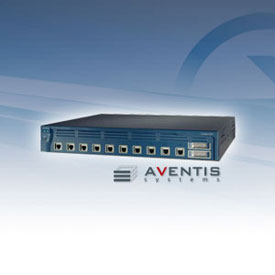
\includegraphics[scale = 1.0]{img/switchL3.jpg}
        \caption{Przełącznik Cisco Catalyst WS-C3550-12T}
    \end{center}
\end{figure}

 \subsection{Przełącznik warstwy 2}
 \textbf{TODO}

 \subsection{Router}
 \textbf{Cisco Router 7200 VXR 7204VXR}
 \begin{itemize}
  	\item \textbf{Ports:} 4 Gigabit Ethernet ports
  	\item \textbf{Speed:} 10/100/1000Mbps
  	\item \textbf{DRAM Memory:} 1GB 
 \end{itemize}
 \begin{figure}[htbp]
	\begin{center}
        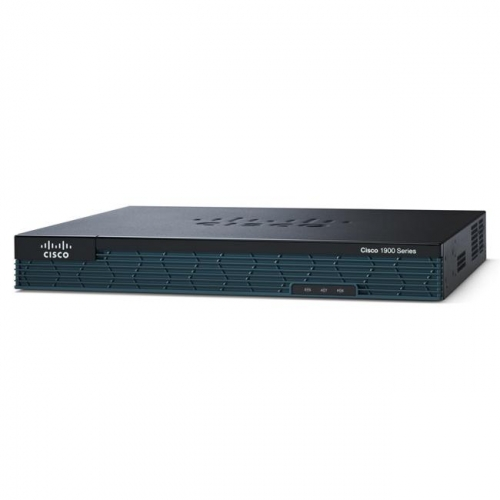
\includegraphics[scale = 0.5]{img/router.jpg}
        \caption{Cisco Router 7200 VXR 7204VXR}
    \end{center}
\end{figure}


\newpage
\subsection{Access Point}
\textbf{Access Point NETGEAR WNCE2001}
\begin{itemize}
	\item \textbf{Standard:} IEEE 802.11n 2.0
	\item \textbf{Ports:} 1 x 10BASE-T/100BASE-TX/1000BASE-T 
\end{itemize}
 \begin{figure}[htbp]
	\begin{center}
        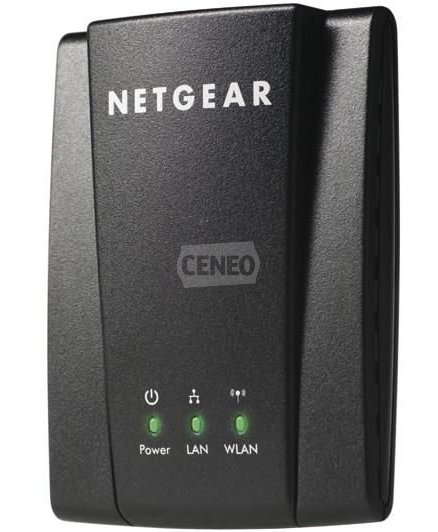
\includegraphics[scale = 0.5]{img/ap.jpg}
        \caption{Access Point NETGEAR WNCE2001}
    \end{center}
\end{figure}